% !TEX root = ../Projektdokumentation.tex
\subsection{Organisation}
\subsubsection{Projektorganisation}
Die Projektorganisation ist wie folgt aufgebaut.

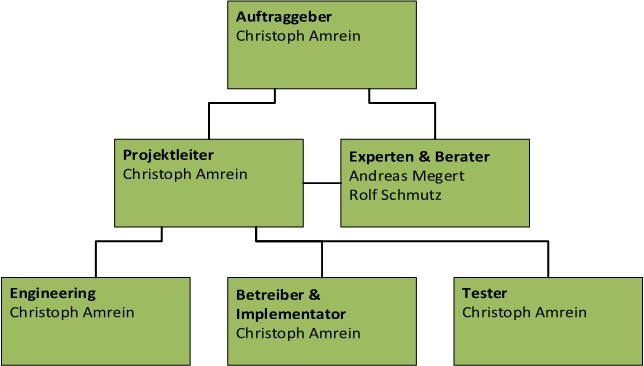
\includegraphics[scale=0.9]{Bilder/Projektorganisation.jpg}{\centering}

\begin{table}[H]
\centering
\begin{tabular}{p{2.5cm}p{13.5cm}}
\hline
\rowcolor{heading}\textbf{Rolle} & \textbf{Verantwortlichkeit} \\\hline
Auftraggeber & Erstellt den Auftrag und übergibt diesen an den Projektleiter \\\hline
Projektleiter & Organisiert die Planung, Durchführung und präsentiert das Projekt. \\\hline
Experte & Stehen in Kontakt mit dem Projektleiter und beraten ihn bei Schwierigkeiten \\\hline
Engineering & Stellt dem Betreiber zu implementierende Applikationen zur Verfügung \\\hline
Betreiber & Setzt die Lösung technisch um \\\hline
Tester & Testet die Lösung auf Fehler  \\\hline
\end{tabular}
\caption{Organisation}
\end{table}

\subsubsection{Projektablage}
\begin{table}[H]
\centering
\begin{tabular}{p{1cm}p{4cm}p{11cm}}
\hline
\rowcolor{heading}\textbf{Nr.} & \textbf{Was} & \textbf{Wo} \\\hline
1 & Allgmeine Ablage& wiki.influ.ch \\\hline
2 & Dokumentation & https://github.com/amreinch/Nebula\_AMC \\\hline
3 & Snapshots & Lokal, D:\textbackslash Diplomarbeit\textbackslash CentOS\_works \\\hline
4 & Skripte, Entwürfe & https://github.com/amreinch/OpenHPC\_Install\_Nebula \\\hline
\end{tabular}
\caption{Projektablage}
\end{table}
